\dosecttoc{}
\pagenumbering{Roman} % Numérotation en chiffres romains (i, ii, iii, ...)
\setcounter{page}{1}

\thispagestyle{empty} % pas de numéro de page sur cette page
\begin{tikzpicture}[remember picture, overlay]
    \node[anchor=south west, inner sep=0] at (current page.south west) {
        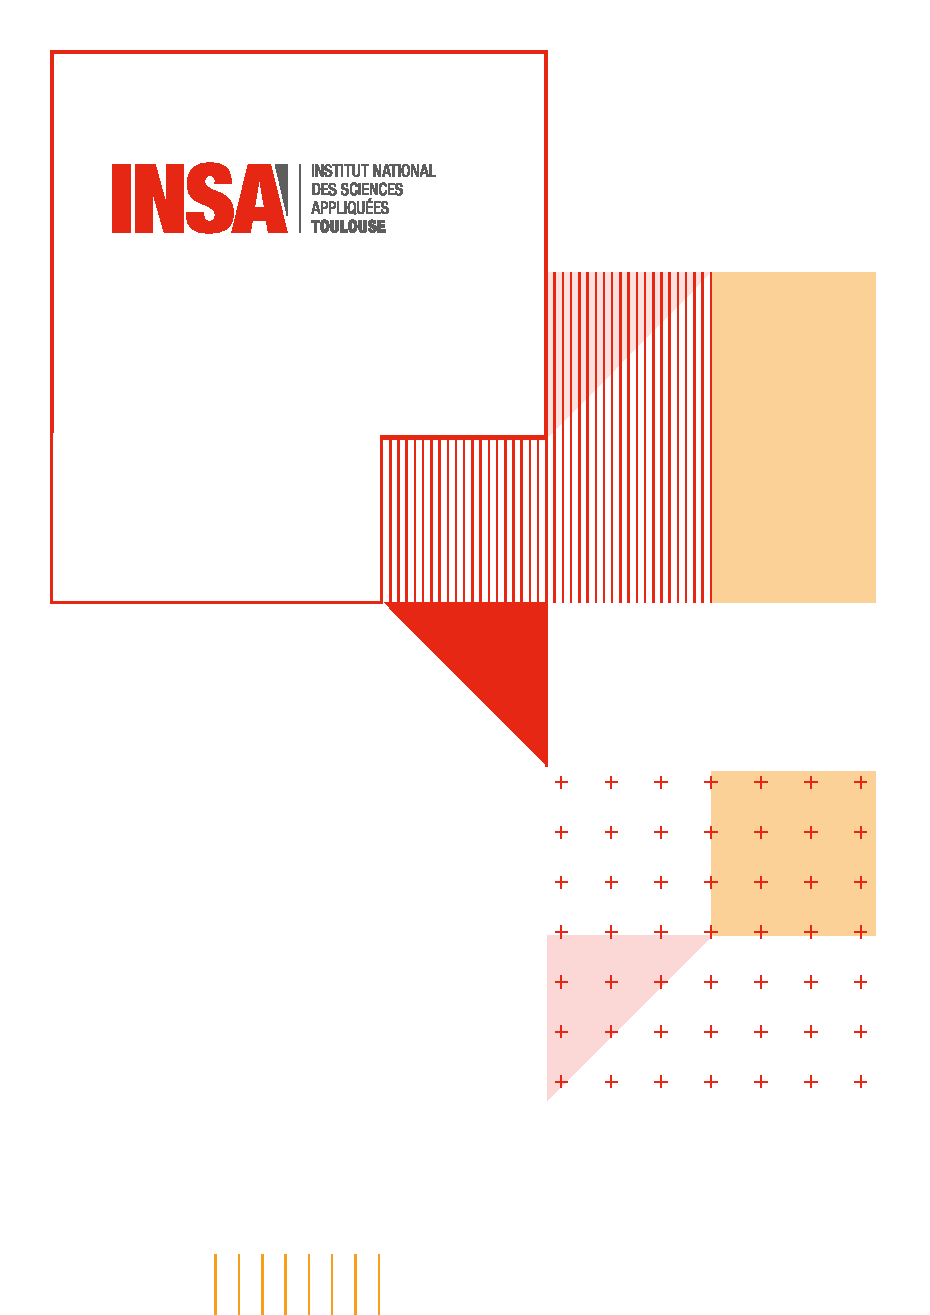
\includegraphics[width=\paperwidth,height=\paperheight]{template/assets/template_first_page.pdf}
    };
    % Ajouter du texte à une position spécifique
    \node at (2.8, -4) {\LARGE \bfseries \MakeUppercase{\titre}};
    \node at (6.8, -7) {\large \firstcouverture};
    \node at (6.8, -17) {\secondcouverture};
    \node at (11.5, -12.2) {\includegraphics[height=3cm]{\imagecouverture}};
\end{tikzpicture}
\newpage
\AddToShipoutPicture{\BackgroundPic} 